\chapter{Functional Progression Prediction: Methods}
\label{ch:study1_methods}

This chapter describes the methodology for Study~I, which develops a patient-level pipeline for predicting short-term functional progression in \gls{ALS}.
Study~II, which replicates and extends a published survival prognosis framework, is described in Chapter~\ref{ch:study2_methods}.

\section{Overview of the Pipeline}
\label{sec:methods_overview}
Study~I treats functional prognosis as binary classification of \textit{rapid} versus \textit{slow} \gls{ALSFRS-R} decline. Each participant contributes one baseline feature vector and one slope outcome for each eligible horizon. The design separates information by time and by participant: predictors are restricted to measurements available at or before the baseline timepoint $t_0$, whereas the target is estimated from assessments collected after $t_0$. Model development is then confined to the development partition, leaving the test partition outside hyperparameter tuning and model selection.

Figure~\ref{fig:pipeline_overview} shows the nine stages of the analysis, from construction of the horizon-specific cohorts to the prototype patient report. Explainability is included because the study examines not only discrimination, but also which baseline measurements drive the fitted model.


\begin{figure}[p]
  \centering
  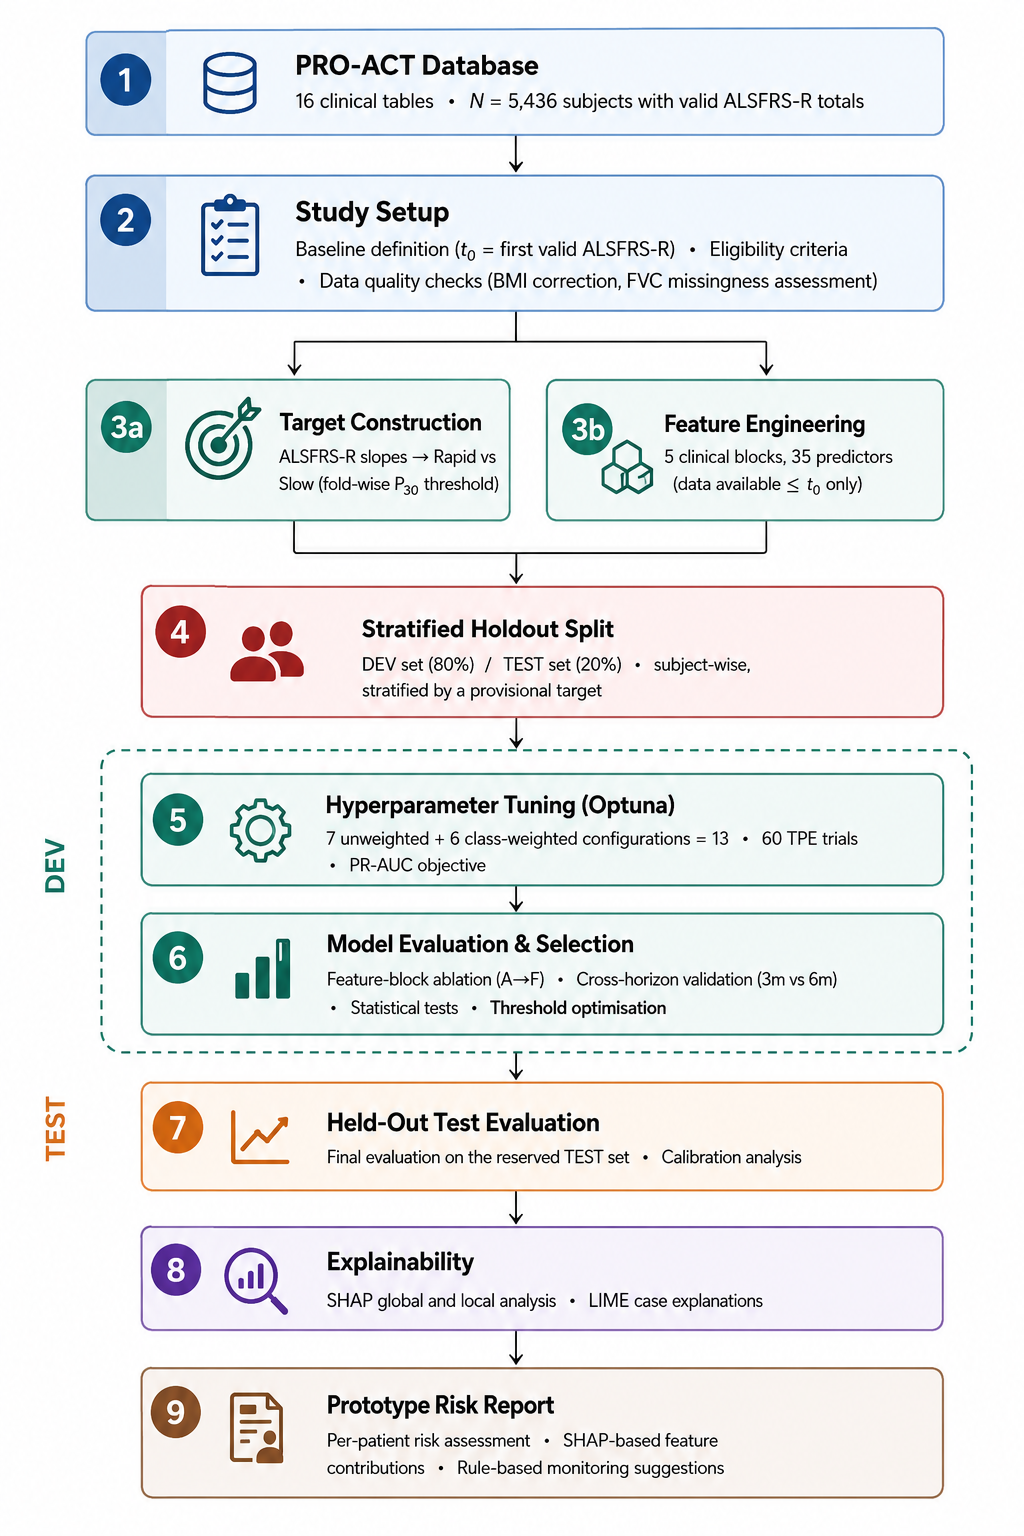
\includegraphics[width=\textwidth,height=0.88\textheight,keepaspectratio]{images/figures/study1_pipeline.png}
  \caption[Study I end-to-end pipeline overview]{Pipeline for Study~I.
  Stages~1--4 construct the horizon-specific datasets and development/test partitions.
  Stages~5--6 use only the development set for cross-validation, hyperparameter optimisation, and model selection.
  Stage~7 evaluates the selected model on the reserved test set, stage~8 examines its predictions using global and local explanation methods, and stage~9 produces a prototype patient-level report.}
  \label{fig:pipeline_overview}
\end{figure}

\clearpage
\section{Dataset}
\label{sec:methods_dataset}
\subsection{PRO-ACT Data Sources}
\label{sec:methods_proact_sources}
Study~I uses the Pooled Resource Open-Access \gls{ALS} Clinical Trials (\gls{PRO-ACT}) database, a public collection of harmonised records from completed ALS clinical trials~\cite{PROACT}. The downloaded extract contains 16 tables covering demographics, clinical assessments, treatments, laboratory results, and other longitudinal measurements. The analysis starts from the 5,436 participants with at least one non-missing \gls{ALSFRS-R} total score; participants represented only in other tables cannot contribute to the functional-progression target.

Eight source tables contribute to the final analytical dataset:
\begin{itemize}
  \item \textbf{\gls{ALSFRS-R}:} longitudinal functional assessments (used for baseline anchoring and target construction),
  \item \textbf{Demographics:} age, sex, ethnicity, and race,
  \item \textbf{Vital Signs:} weight, height, \gls{BMI}, pulse, respiratory rate, temperature, and blood pressure variants (systolic, diastolic, standing, supine),
  \item \textbf{\gls{FVC}:} forced vital capacity measurements (litres, percent of normal) as a marker of respiratory function,
  \item \textbf{Riluzole:} riluzole exposure recorded at or before baseline,
  \item \textbf{Treatment:} clinical-trial treatment arm,
  \item \textbf{Concomitant Medications:} number of distinct medications recorded at or before baseline,
  \item \textbf{Labs:} serum creatinine and alanine aminotransferase (\gls{ALT}).
\end{itemize}
The feature set is restricted to variables present in this extract and available near baseline. Imaging, genetic, and electrophysiological measurements are not part of the analysed tables and are therefore outside the scope of the study.

\subsection{Study Population and Eligibility}
\label{sec:methods_population}
Baseline is defined separately for each participant as the date of the first valid \gls{ALSFRS-R} total score. Eligibility is then assessed independently for the 90- and 180-day horizons. A participant is retained for a given horizon when:
\begin{enumerate}
  \item a valid baseline score and date are available;
  \item at least one assessment falls within the endpoint band $[t_0+H-7,\;t_0+H+7]$; and
  \item the observations from $t_0$ to $t_0+H+7$ contain at least two distinct assessment times, allowing a slope to be estimated.
\end{enumerate}

Three or more observations were preferred for a more stable slope estimate, but this was monitored as a quality indicator rather than imposed as an exclusion criterion. The resulting cohorts contain 2,407 participants at three months and 1,392 at six months. Of these, 720 appear in both cohorts. The horizons are analysed as separate prediction tasks, with their own slopes, labels, and data partitions; no performance estimate combines observations from the two analyses. The smaller six-month cohort mainly reflects the requirement for an assessment within seven days of day~180.
Figure~\ref{fig:consort_flowchart} summarises the cohort derivation.

\begin{figure}[ht!]
  \centering
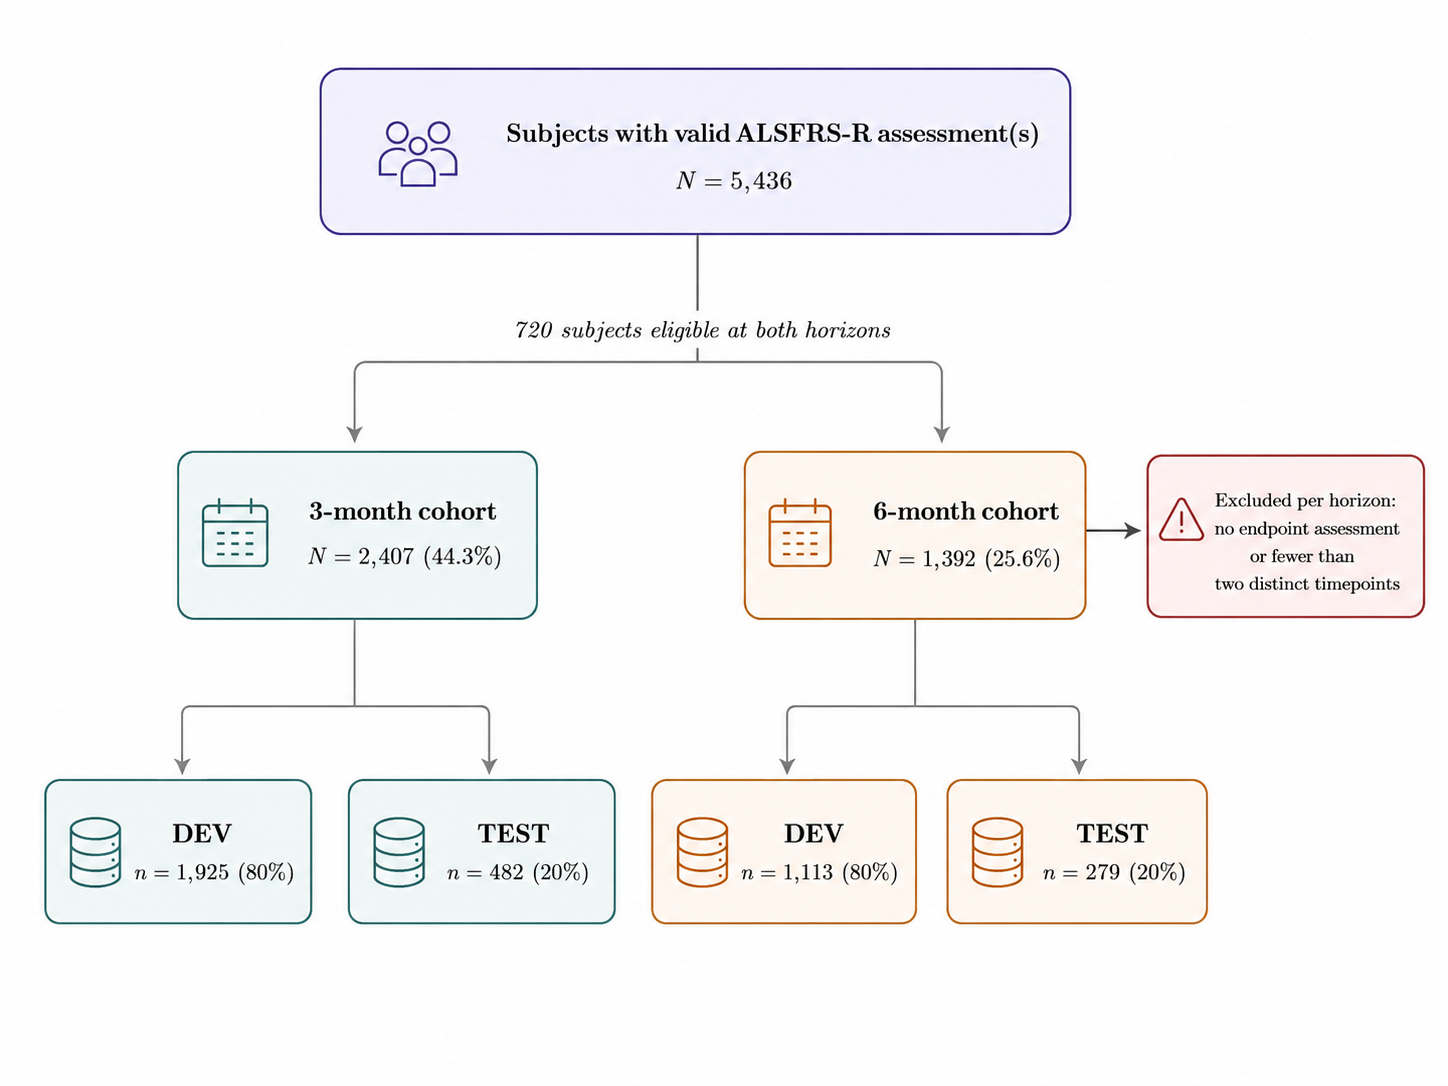
\includegraphics[width=\textwidth,height=0.82\textheight,keepaspectratio]{images/figures/study1_cohort_derivation.png}
  \caption[Cohort derivation by prediction horizon]{Derivation of the Study~I cohorts from the 5,436 participants with at least one valid ALSFRS-R assessment.
  Eligibility is evaluated separately at three and six months according to the availability of repeated assessments and an endpoint measurement within the corresponding $\pm7$-day band.
  Each horizon-specific cohort is subsequently divided into development (DEV, 80\%) and test (TEST, 20\%) partitions.}
  \label{fig:consort_flowchart}
\end{figure}

\subsection{Held-Out Data Partitioning}
\label{sec:methods_holdout}
Before model development, each horizon-specific cohort is divided into development (\gls{DEV}, 80\%) and test (\gls{TEST}, 20\%) partitions with a fixed random seed. Stratification uses a provisional rapid/slow label obtained from the 30th percentile of the complete horizon-specific slope distribution. This provisional label is used only to preserve the approximate class proportion in the split. It is not used for training or final evaluation: after partitioning, the operative slope threshold is recomputed from \gls{DEV} data and then applied unchanged to \gls{TEST}.

The six-month partition contains 1,113 development and 279 test participants; the three-month partition contains 1,925 and 482, respectively. Cross-validation, preprocessing, hyperparameter optimisation, ablation, threshold selection, and model selection use the \gls{DEV} partition only. The \gls{TEST} partition is accessed after these choices have been fixed to estimate final performance (Section~\ref{sec:results_test_eval}).

\section{Baseline Definition and Leakage-Free Protocol}
\label{sec:methods_baseline}
\subsection{Baseline Timepoint ($t_0$)}
\label{sec:methods_t0}
For each subject, the baseline timepoint $t_0$ is the earliest recorded day with a non-missing \gls{ALSFRS-R} total score. This definition gives every trajectory a reproducible starting point without requiring participants to survive or remain under observation until a later visit. Of the 5,436 subjects in the initial analytical pool, 4,144 (76.2\%) have their first valid score at the \gls{PRO-ACT} reference day ($\Delta=0$); for the remainder, $t_0$ is the earliest valid assessment available in their record. The reference day should therefore be understood as a database time origin rather than an exact proxy for diagnosis or symptom onset.

\subsection{Why Baseline Matters}
\label{sec:methods_baseline_why}
The prediction task is anchored at $t_0$. Predictors are constructed from information recorded at or before this point, whereas later observations are used only to derive the outcome. The baseline \gls{ALSFRS-R} score is an exception only in appearance: it is available at prediction time and is also the first observation in the subsequent slope calculation. No measurement recorded after $t_0$ is used as a predictor. This prevents future laboratory, respiratory, or functional measurements from entering the feature set and inflating performance. Figure~\ref{fig:temporal_separation} shows the resulting temporal arrangement for both horizons.

\begin{figure}[ht!]
  \centering
  \begin{tikzpicture}[
    >=Stealth,
    tlabel/.style={font=\scriptsize, text=black!70},
    blabel/.style={font=\scriptsize\bfseries},
  ]

  % ── Dimensions ──
  \def\tlength{14}   % total timeline length in cm
  \def\tzero{3.5}    % position of t0
  \def\yrow{0}       % y for 6-month row
  \def\yrowB{-2.8}   % y for 3-month row

  % ======================================================================
  %  6-MONTH HORIZON
  % ======================================================================
  \node[blabel, anchor=east] at (-0.3, \yrow) {6-month};

  % Main timeline axis
  \draw[->, black!40, line width=0.6pt]
    (0,\yrow) -- (\tlength,\yrow)
    node[right, tlabel] {time (days)};

  % ── Feature zone: data ≤ t0 ──
  \fill[blue!12] (0,\yrow-0.35) rectangle (\tzero,\yrow+0.35);
  \draw[blue!50!black, line width=0.4pt]
    (0,\yrow-0.35) rectangle (\tzero,\yrow+0.35);
  \node[font=\scriptsize, text=blue!60!black] at (\tzero/2, \yrow)
    {Features (data $\leq t_0$)};

  % ── t0 marker ──
  \draw[black, line width=1pt] (\tzero,\yrow-0.55) -- (\tzero,\yrow+0.55);
  \node[font=\small\bfseries, above] at (\tzero,\yrow+0.55) {$t_0$};

  % ── Target zone: 6m ──
  % H = 180d → position at tzero + 7.0cm ; tolerance ±7d → ±0.28cm
  \def\sixmEnd{10.5}       % t0 + 180d
  \def\tolW{0.28}          % ±7d tolerance half-width

  \fill[orange!12]
    (\tzero,\yrow-0.35) rectangle (\sixmEnd+\tolW,\yrow+0.35);
  \draw[orange!50!black, line width=0.4pt]
    (\tzero,\yrow-0.35) rectangle (\sixmEnd+\tolW,\yrow+0.35);
  \node[font=\scriptsize, text=orange!60!black]
    at ({(\tzero+\sixmEnd+\tolW)/2}, \yrow)
    {Target window (ALSFRS-R slope)};

  % Tolerance band shading
  \fill[red!10] (\sixmEnd-\tolW,\yrow-0.35) rectangle (\sixmEnd+\tolW,\yrow+0.35);
  \draw[red!40, dashed, line width=0.4pt]
    (\sixmEnd-\tolW,\yrow-0.35) -- (\sixmEnd-\tolW,\yrow+0.35);
  \draw[red!40, dashed, line width=0.4pt]
    (\sixmEnd+\tolW,\yrow-0.35) -- (\sixmEnd+\tolW,\yrow+0.35);

  % 180d label
  \draw[black!50, line width=0.5pt] (\sixmEnd,\yrow-0.55) -- (\sixmEnd,\yrow+0.55);
  \node[font=\scriptsize, above] at (\sixmEnd, \yrow+0.55) {$t_0\!+\!180$d};

  % Tolerance annotation
  \draw[<->, red!50!black, line width=0.4pt]
    (\sixmEnd-\tolW, \yrow-0.55) -- (\sixmEnd+\tolW, \yrow-0.55)
    node[midway, below, font=\tiny, text=red!50!black] {$\pm 7$d};

  % ── Forbidden zone label ──
  \node[font=\tiny, text=red!50!black, rotate=90, anchor=south]
    at (\tzero+0.15, \yrow) {};

  % ── Leakage barrier ──
  \draw[red!70!black, line width=1.2pt, densely dashed]
    (\tzero, \yrow-0.7) -- (\tzero, \yrow+0.85);
  \node[font=\tiny\bfseries, text=red!60!black, above right]
    at (\tzero+0.05, \yrow+0.6) {leakage barrier};

  % Example data points (features)
  \foreach \x in {0.6, 1.3, 2.1, 2.8, 3.3} {
    \fill[blue!60!black] (\x, \yrow+0.15) circle (1.5pt);
  }
  % Example data points (target)
  \foreach \x in {4.5, 5.8, 7.0, 8.2, 9.5, 10.3} {
    \fill[orange!70!black] (\x, \yrow+0.15) circle (1.5pt);
  }

  % ======================================================================
  %  3-MONTH HORIZON
  % ======================================================================
  \node[blabel, anchor=east] at (-0.3, \yrowB) {3-month};

  % Main timeline axis
  \draw[->, black!40, line width=0.6pt]
    (0,\yrowB) -- (\tlength,\yrowB)
    node[right, tlabel] {time (days)};

  % ── Feature zone ──
  \fill[blue!12] (0,\yrowB-0.35) rectangle (\tzero,\yrowB+0.35);
  \draw[blue!50!black, line width=0.4pt]
    (0,\yrowB-0.35) rectangle (\tzero,\yrowB+0.35);
  \node[font=\scriptsize, text=blue!60!black] at (\tzero/2, \yrowB)
    {Features (data $\leq t_0$)};

  % ── t0 marker ──
  \draw[black, line width=1pt] (\tzero,\yrowB-0.55) -- (\tzero,\yrowB+0.55);
  \node[font=\small\bfseries, above] at (\tzero,\yrowB+0.55) {$t_0$};

  % ── Target zone: 3m ──
  \def\threemEnd{7.0}    % t0 + 90d

  \fill[teal!12]
    (\tzero,\yrowB-0.35) rectangle (\threemEnd+\tolW,\yrowB+0.35);
  \draw[teal!50!black, line width=0.4pt]
    (\tzero,\yrowB-0.35) rectangle (\threemEnd+\tolW,\yrowB+0.35);
  \node[font=\scriptsize, text=teal!60!black]
    at ({(\tzero+\threemEnd+\tolW)/2}, \yrowB)
    {Target window};

  % Tolerance band
  \fill[red!10] (\threemEnd-\tolW,\yrowB-0.35) rectangle (\threemEnd+\tolW,\yrowB+0.35);
  \draw[red!40, dashed, line width=0.4pt]
    (\threemEnd-\tolW,\yrowB-0.35) -- (\threemEnd-\tolW,\yrowB+0.35);
  \draw[red!40, dashed, line width=0.4pt]
    (\threemEnd+\tolW,\yrowB-0.35) -- (\threemEnd+\tolW,\yrowB+0.35);

  % 90d label
  \draw[black!50, line width=0.5pt] (\threemEnd,\yrowB-0.55) -- (\threemEnd,\yrowB+0.55);
  \node[font=\scriptsize, above] at (\threemEnd, \yrowB+0.55) {$t_0\!+\!90$d};

  % Tolerance annotation
  \draw[<->, red!50!black, line width=0.4pt]
    (\threemEnd-\tolW, \yrowB-0.55) -- (\threemEnd+\tolW, \yrowB-0.55)
    node[midway, below, font=\tiny, text=red!50!black] {$\pm 7$d};

  % ── Leakage barrier ──
  \draw[red!70!black, line width=1.2pt, densely dashed]
    (\tzero, \yrowB-0.7) -- (\tzero, \yrowB+0.85);

  % Example data points (features)
  \foreach \x in {0.6, 1.3, 2.1, 2.8, 3.3} {
    \fill[blue!60!black] (\x, \yrowB+0.15) circle (1.5pt);
  }
  % Example data points (target)
  \foreach \x in {4.2, 5.2, 6.1, 6.8} {
    \fill[teal!70!black] (\x, \yrowB+0.15) circle (1.5pt);
  }

  % ======================================================================
  %  LEGEND
  % ======================================================================
  \node[font=\scriptsize, anchor=west] at (0, \yrowB-1.2) {
    \tikz{\fill[blue!60!black] (0,0) circle (1.5pt);}\ Clinical measurement (feature)
    \quad
    \tikz{\fill[orange!70!black] (0,0) circle (1.5pt);}\ ALSFRS-R measurement (target)
    \quad
    \tikz{\draw[red!70!black, line width=1pt, densely dashed] (0,0) -- (0.5,0);}\ Leakage barrier
  };

  \end{tikzpicture}
  \caption[Feature--target temporal separation diagram]{Temporal separation between feature extraction and target construction.
  For each subject, features are derived from data available up to and including~$t_0$ (blue zone), while the target slope uses ALSFRS-R measurements from~$t_0$ onwards (orange/teal zone).
  The dashed red line marks the boundary beyond which measurements cannot be used as predictors.
  At least one ALSFRS-R assessment must fall within the $\pm 7$-day endpoint band (red shading).
  Blue and coloured dots represent example clinical measurements for a hypothetical patient.}
  \label{fig:temporal_separation}
\end{figure}

\section{Target Construction: ALSFRS-R Slopes}
\label{sec:methods_targets}
\subsection{Horizon Definition and Temporal Tolerance}
\label{sec:methods_horizons}
Two prediction horizons are considered:
\begin{itemize}
  \item \textbf{3 months:} $H=90$ days with tolerance $\pm 7$ days,
  \item \textbf{6 months:} $H=180$ days with tolerance $\pm 7$ days.
\end{itemize}
For a subject to be eligible at horizon $H$, at least one \gls{ALSFRS-R} assessment must occur between $t_0+H-7$ and $t_0+H+7$ days. The slope is then fitted using all available assessments from $t_0$ through $t_0+H+7$ days. This endpoint band allows modest variation in visit timing while ensuring that the fitted trajectory reaches the intended horizon.

The six-month horizon is treated as the primary analysis because its slopes are estimated from more observations per subject (median seven, compared with four at three months) and over a longer interval. The three-month analysis is retained as a shorter-horizon comparison, and its predictive performance is evaluated using the same modelling protocol.

\subsection{Slope Estimation}
\label{sec:methods_slope}
Functional progression is represented by the change in total \gls{ALSFRS-R} score over time, a common functional outcome in \gls{ALS} prognostic research~\cite{Pancotti2022, Anani2023}. For subject $i$, ordinary least squares regression is fitted separately at each eligible horizon:
\[
  \mathrm{ALSFRS\mbox{-}R}_{ij}
  = \beta_{0i} + \beta_{1i}(t_{ij}-t_{0i}) + \varepsilon_{ij},
\]
where $t_{ij}$ is the day of assessment $j$. At least two distinct assessment days are required. The fitted coefficient $\hat{\beta}_{1i}$ is expressed in points per day and rescaled to points per 30 days:
\[
  \mathrm{slope}_{30,i}=30\hat{\beta}_{1i}.
\]
A negative value denotes functional decline, with increasingly negative slopes indicating faster observed deterioration. This summary assumes that the trajectory is approximately linear within the 90- or 180-day window; it does not attempt to model shorter-term fluctuations or non-linear change.

The number of assessments contributing to each slope and the presence of an endpoint-band measurement are retained as quality indicators. They are not additional exclusion criteria beyond the requirement for two distinct timepoints and an endpoint observation. In the six-month cohort, 99.8\% of slopes are based on at least three assessments and the median is seven. The corresponding values at three months are 90.5\% and four assessments.

\subsection{Binary Target: Rapid vs Slow Progression}
\label{sec:methods_binary_target}
The continuous slope is converted into a binary classification target. The positive class, \textit{rapid}, comprises the 30\% most negative slopes; the remaining observations are labelled \textit{slow}. The latter term is retained for consistency throughout the study, although it denotes the non-rapid 70\% rather than a separately validated clinical phenotype.

The 30th percentile is an operational choice rather than an established clinical cutoff. It focuses the task on the faster-declining tail while retaining enough positive observations for model development and allowing the effect of class weighting to be examined. Within cross-validation, the percentile is calculated from the training slopes only and the resulting numerical cutoff is applied unchanged to the validation slopes (Section~\ref{sec:methods_validation}). The validation prevalence can therefore differ slightly from 30\%. For final held-out evaluation, one cutoff is derived from the complete \gls{DEV} partition and applied to \gls{TEST}.

Across the full six-month cohort, the descriptive 30th percentile is $-1.25$ points per 30 days. This value is shown in Figure~\ref{fig:slope_histogram_6m} to make the target definition tangible, but it is not used to label the held-out test set.

\begin{figure}[ht!]
  \centering
  
\includegraphics[width=0.85\linewidth]{images/figures/slope_histogram_6m.png}
  \caption[ALSFRS-R slope distribution, 6-month cohort]{Distribution of ALSFRS-R slopes (points/30\,days) for the 6-month cohort ($N\!=\!1{,}392$).
  The dashed line marks the 30th-percentile cutoff ($-1.25$\,points/month); subjects to the left (red) are labelled \textit{rapid}, those to the right (blue) \textit{slow}.
  The cutoff shown is computed on the full cohort for illustration. Training-fold cutoffs are used during cross-validation, and the cutoff used for final evaluation is calculated from the DEV partition only.}
  \label{fig:slope_histogram_6m}
\end{figure}

\section{Feature Engineering at Baseline ($t_0$)}
\label{sec:methods_features}
\subsection{Feature Blocks}
\label{sec:methods_feature_blocks}
The model uses 35 predictors grouped into five clinical blocks:
\begin{itemize}
  \item \textbf{Baseline} ($n\!=\!15$): age, sex, ethnicity, seven race indicators, total \gls{ALSFRS-R}, its three respiratory items, and mode of administration;
  \item \textbf{Vitals} ($n\!=\!12$): weight, height, \gls{BMI}, pulse, respiratory rate, temperature, and six blood-pressure measurements;
  \item \textbf{Respiratory} ($n\!=\!3$): best \gls{FVC} in litres, best percentage of normal, and the recorded subject-normal value;
  \item \textbf{Treatment} ($n\!=\!3$): pre-baseline riluzole use, clinical-trial study arm, and number of concomitant medications recorded before baseline;
  \item \textbf{Laboratory} ($n\!=\!2$): creatinine and \gls{ALT}.
\end{itemize}
The subject identifier, three temporal offsets, both horizon-specific slopes, and \texttt{ALSFRS\_Responded\_By} are excluded from the model matrix. The slopes are outcomes rather than predictors; the offsets are retained only to verify temporal selection; and the response-source field is missing for more than 93\% of the cohort. Table~\ref{tab:feature_summary} lists the predictors, their data types, and their coverage in the six-month cohort. The same block definitions are used in the ablation analysis (Section~\ref{sec:methods_ablation}).

\begin{table}[ht!]
\centering
\caption{Complete feature set (v2): 35 predictors grouped by clinical block.
Coverage denotes the percentage of 6-month cohort subjects ($N\!=\!1{,}392$) with a non-missing value.
\textit{Type} distinguishes numeric features (median-imputed) from categorical features (most-frequent imputed, then one-hot encoded).}
\label{tab:feature_summary}
\footnotesize
\begin{tabular}{r l l c r}
\toprule
\# & Feature & Block & Type & Cover.\ (\%) \\
\midrule
 1 & ALSFRS-R total ($t_0$)       & Baseline & Num & 100.0 \\
 2 & Age                           & Baseline & Num &  87.1 \\
 3 & Sex                           & Baseline & Cat & 100.0 \\
 4 & Ethnicity                     & Baseline & Cat &  62.4 \\
 5 & Race: Caucasian               & Baseline & Bin &  89.7 \\
 6 & Race: Black / African Amer.   & Baseline & Bin &   8.7 \\
 7 & Race: Asian                   & Baseline & Bin &   8.4 \\
 8 & Race: Amer.\ Indian / Alaska  & Baseline & Bin &   7.7 \\
 9 & Race: Hawaiian / Pac.\ Isl.   & Baseline & Bin &   7.3 \\
10 & Race: Other                   & Baseline & Bin &   2.3 \\
11 & Race: Unknown                 & Baseline & Bin &   7.5 \\
12 & R-1 Dyspnea                   & Baseline & Num &  93.8 \\
13 & R-2 Orthopnea                 & Baseline & Num &  93.8 \\
14 & R-3 Respiratory Insufficiency  & Baseline & Num &  93.8 \\
15 & Mode of Administration         & Baseline & Cat &  17.0 \\
\cmidrule{1-5}
16 & Weight (kg)                    & Vitals   & Num &  79.2 \\
17 & Height (cm)                    & Vitals   & Num &  44.9 \\
18 & BMI                            & Vitals   & Num &  44.3 \\
19 & Pulse                          & Vitals   & Num &  71.8 \\
20 & Respiratory Rate               & Vitals   & Num &  66.8 \\
21 & Temperature                    & Vitals   & Num &  66.6 \\
22 & BP Systolic                    & Vitals   & Num &  71.9 \\
23 & BP Diastolic                   & Vitals   & Num &  71.9 \\
24 & Standing BP Systolic           & Vitals   & Num &   5.5 \\
25 & Standing BP Diastolic          & Vitals   & Num &   5.5 \\
26 & Supine BP Systolic             & Vitals   & Num &   5.5 \\
27 & Supine BP Diastolic            & Vitals   & Num &   5.5 \\
\cmidrule{1-5}
28 & FVC (litres)                   & FVC      & Num &  56.3 \\
29 & FVC (\% of normal)             & FVC      & Num &  54.5 \\
30 & Subject normal (litres)        & FVC      & Num &  33.3 \\
\cmidrule{1-5}
31 & Riluzole use (pre-$t_0$)       & Treatment & Bin & 100.0 \\
32 & Study arm                      & Treatment & Cat &  91.1 \\
33 & No.\ concomitant medications   & Treatment & Num & 100.0 \\
\cmidrule{1-5}
34 & ALT (SGPT)                     & Labs     & Num &  69.0 \\
35 & Creatinine                     & Labs     & Num &  64.7 \\
\bottomrule
\end{tabular}
\par\smallskip
{\scriptsize Num = numeric; Cat = categorical (one-hot encoded); Bin = binary indicator.
Coverage for race indicators reflects the fraction of subjects for whom that specific race field was recorded in the source database.}
\end{table}


\subsection{Temporal Selection Rule (Last Pre-Baseline)}
\label{sec:methods_last_prebaseline}
Only records dated at or before $t_0$ are eligible for feature construction. For vital signs and \gls{FVC}, the most recent eligible record is selected for each subject. Weight and height are converted to kilograms and centimetres, respectively, and \gls{BMI} is calculated from those converted values. The FVC features are taken from the latest eligible test and use the highest value across the available trials at that visit.

Laboratory values are selected separately for each test, using the most recent creatinine and \gls{ALT} result at or before $t_0$. Riluzole is encoded as one when a record confirms use by baseline and zero otherwise. The concomitant-medication feature counts distinct coded medications with a start date no later than $t_0$; subjects with no qualifying record receive a count of zero. Study arm is treated as a trial-level baseline attribute. Missing values are retained when no eligible measurement is available and are handled within the preprocessing pipeline (Section~\ref{sec:methods_preprocessing}).

\subsection{Coverage and Missingness}
\label{sec:methods_coverage}
Coverage is defined as the proportion of the six-month cohort with a non-missing value. It varies considerably within blocks. Total \gls{ALSFRS-R} and sex are complete, age is available for 87.1\%, and the three respiratory scale items for 93.8\%; by contrast, mode of administration is recorded for only 17.0\%. At least one vital-sign feature is present for 80.6\% of subjects, but individual coverage ranges from 79.2\% for weight to 5.5\% for standing and supine blood-pressure fields.

FVC in litres is available for 56.3\% of subjects, percentage of normal for 54.5\%, and the subject-normal value for 33.3\%. At least one of the three respiratory features is present for 60.7\% of the cohort. Study arm is available for 91.1\%, while the operationally constructed riluzole indicator and medication count contain no missing values. Creatinine and \gls{ALT} coverage is 64.7\% and 69.0\%, respectively. These differences are reported per feature in Table~\ref{tab:feature_summary} and motivate the fold-specific imputation described later.

\subsection{FVC Missingness Analysis}
\label{subsec:methods_fvc_missingness}
Because FVC in litres is absent for 43.7\% of the six-month cohort, participants with and without a valid baseline value are compared across 11 observed variables. Continuous distributions use two-sided Mann--Whitney~$U$ tests with absolute Cohen's~$d$ effect sizes; categorical variables use Pearson's $\chi^2$ test with Cram\'er's~$V$. Raw $p$-values are interpreted against a Bonferroni threshold of $0.05/11=0.0045$. These comparisons can identify observed differences but cannot establish that the data are \gls{MAR} or exclude an \gls{MNAR} component. Appendix~\ref{app:fvc_missingness} provides the variables, complete results, and effect-size definition.

\subsection{Data Quality: BMI Correction}
\label{sec:methods_bmi_correction}
During baseline feature construction, height values outside $[120,220]$\,cm and weight values outside $[30,200]$\,kg were set to \texttt{NaN}. The anomalous heights were compatible with a misplaced decimal point, but the intended values could not be verified from the source data; treating them as missing avoids introducing an assumed correction. This rule affected 132 selected height measurements and 31 weights. \gls{BMI} was recalculated only when both measurements remained valid, with missing values subsequently handled within the model pipeline. Appendix~\ref{app:bmi_correction} documents the original records and the checks performed after cleaning.

\section{Exploratory Analysis: Treatment Variables and Progression}
\label{sec:methods_eda_treatment}
The treatment block is examined descriptively before modelling using the complete six-month cohort and a rapid-progression label based on the global 30th-percentile slope cutoff. Active and Placebo arms, as well as participants with and without documented pre-baseline riluzole use, are compared using a $\chi^2$ test for the binary label and a two-sided Mann--Whitney~$U$ test for the continuous slope. Medication burden and the most frequently recorded pre-baseline drugs are summarised without drug-level hypothesis testing. This exploratory label is not used during model development, where cutoffs remain derived from the training data.

These variables cannot support treatment-effect claims in the pooled \gls{PRO-ACT} data. ``Active'' combines different experimental interventions, riluzole exposure is observational, and medication count may reflect comorbidity, symptom management, trial procedures, or recording intensity. The complete protocol and descriptive outputs are provided in Appendix~\ref{app:treatment_eda}; the findings retained in the main analysis are reported in Section~\ref{sec:results_eda_treatment}.

\section{Modelling Setup}
\label{sec:methods_modeling}
\subsection{Models Considered}
\label{sec:methods_models}
Seven supervised learning algorithms were selected to compare model families with different assumptions about the structure of the data:
\begin{itemize}
  \item \textbf{K-Nearest Neighbours (\gls{KNN}):} a non-parametric, distance-based classifier included as a simple local-learning baseline.
  \item \textbf{Decision Tree (\gls{DT}):} a single-tree classifier that provides an interpretable comparison with the tree ensembles.
  \item \textbf{Random Forest (\gls{RF}):} a bagging ensemble used to assess whether averaging multiple trees improves on a single decision tree.
  \item \textbf{Support Vector Machine (\gls{SVM}):} a maximum-margin classifier for which both linear and \gls{RBF} kernels were considered during optimisation.
  \item \textbf{Logistic Regression (\gls{LR}):} a linear probabilistic model retained as an interpretable baseline and for subsequent coefficient analysis.
  \item \textbf{LightGBM (\gls{LGBM}):} a histogram-based gradient-boosting implementation designed for tabular data.
  \item \textbf{XGBoost (\gls{XGB}):} a regularised gradient-boosting implementation that also supports the planned \gls{SHAP} analysis.
\end{itemize}
Together, these algorithms cover local, linear, kernel-based, bagging, and boosting approaches. Neural-network architectures were not included because the analysis focused on established methods for moderate-sized tabular clinical data and required a tractable comparison across model families. This choice defines the scope of the comparison rather than implying that neural networks cannot be applied to this dataset.
Following hyperparameter optimisation (Section~\ref{sec:methods_optuna}), the final model is selected using cross-validated \gls{PR-AUC}. Its predictions are examined using \gls{SHAP} (Section~\ref{sec:methods_xai_plan}), while Logistic Regression provides a complementary coefficient-based analysis.

\subsection{Preprocessing Pipeline}
\label{sec:methods_preprocessing}
The 35 predictors comprise 31 numeric and four categorical variables: sex, ethnicity, mode of administration, and study arm. A common preprocessing structure is used across models:
\begin{itemize}
  \item Numeric variables are imputed using the training-fold median. They are then standardised using \texttt{StandardScaler} for \gls{KNN}, \gls{LR}, and \gls{SVM}.
  \item Categorical variables are imputed using the most frequent training-fold category and one-hot encoded. Categories not observed during fitting are ignored when new data are transformed.
\end{itemize}
Median imputation provides a simple and reproducible treatment of the uneven feature coverage without estimating additional multivariable imputation models from this moderate-sized cohort. It does not resolve possible informative missingness, particularly for FVC, and this limitation is considered alongside the missingness analysis in Section~\ref{sec:results_fvc_missingness}. Both numeric and categorical imputers are fitted within each training fold rather than on the complete dataset.
The categorical variables contain between two and four observed levels. One-hot encoding is therefore practical and avoids imposing an ordinal relationship between categories. Decision Tree, Random Forest, LightGBM, and XGBoost use the same imputation and encoding steps but do not use numeric standardisation.
The preprocessing transformer and classifier are combined in a \texttt{scikit-learn} \texttt{Pipeline}. Within each cross-validation fold, this pipeline is fitted only on the training partition and then applied to the held-out fold. Imputation values, scaling parameters, and encoded categories are therefore estimated without access to the validation data.

\subsection{Software and Computational Environment}
\label{sec:methods_environment}
The analysis was implemented in Python~3.12.10 on Windows~11. The main library versions were \texttt{scikit-learn}~1.8.0, \texttt{XGBoost}~3.2.0, \texttt{LightGBM}~4.6.0, \texttt{Optuna}~4.7.0, \texttt{SHAP}~0.50.0, \texttt{LIME}~0.2.0.1, \texttt{pandas}~3.0.1, \texttt{NumPy}~2.4.2, and \texttt{joblib}~1.5.3. The training scripts used \gls{CPU} implementations and did not request \gls{GPU} acceleration.
For the six-month horizon, the 13 model and class-weight configurations required 3,900 cross-validation fits during the 60-trial Optuna searches. The recorded optimisation time totalled approximately 34 minutes, with individual configurations ranging from 8 to 768 seconds. These timings describe the workstation used for this analysis and are not intended as hardware-independent benchmarks.

\section{Handling Class Imbalance}
\label{sec:methods_imbalance}
The rapid-progression class represents approximately 30\% of the development cohort, corresponding to a class ratio of about 1:2.3. To examine whether this imbalance affects the fitted models, each classifier is evaluated with and without cost-sensitive weighting. \gls{KNN} does not provide native class weighting and is therefore evaluated only in its standard form, giving 13 model--mode configurations in total.

In the unbalanced mode, both classes retain the model's default contribution to the training objective. In the balanced mode, the weighting is applied separately within each training fold:
\begin{itemize}
  \item Decision Tree, Random Forest, \gls{SVM}, and Logistic Regression use \texttt{class\_weight=balanced}, which assigns weights inversely proportional to the class frequencies in the training data;
  \item LightGBM uses \texttt{is\_unbalance=True}; and
  \item XGBoost uses \texttt{scale\_pos\_weight} set to $n_{\mathrm{negative}}/n_{\mathrm{positive}}$ in the corresponding training fold.
\end{itemize}
Validation-fold labels and class counts are not used to determine these weights.

\gls{PR-AUC}, implemented as average precision, is the primary optimisation and model-ranking metric because it summarises the precision--recall trade-off for the minority class without requiring a decision threshold. \gls{ROC-AUC} is reported as a secondary threshold-free measure. During model comparison, $F_1$ and $F_2$ are calculated at the default threshold of 0.5 for descriptive purposes only and do not determine the selected model. Spearman correlations across the 13 configurations are used to compare the rankings produced by the threshold-free and fixed-threshold metrics.

The operating threshold is selected only after model selection, using out-of-fold predictions from the development set as described in Section~\ref{sec:methods_threshold_final}. Synthetic over- or under-sampling is not used in Study~I; the imbalance analysis is restricted to the native weighting options above so that every model is trained on the observed development records.

\section{Evaluation Metrics}
\label{sec:methods_metrics}
Performance is assessed using complementary threshold-free, threshold-dependent, and probability-based measures. All classification metrics treat rapid progression as the positive class. Table~\ref{tab:metrics} summarises the measures used, where $P$ denotes precision, $R$ recall, TP true positives, FP false positives, FN false negatives, $p_i$ the predicted probability for subject~$i$, and $y_i \in \{0,1\}$ the observed label.

\gls{PR-AUC} is implemented using \texttt{average\_precision\_score}. Average precision forms a stepwise summary of the precision--recall curve and gives greater weight to improvements in recall achieved at high precision. Its no-skill reference depends on the proportion of rapid progressors, which is approximately 0.30 in this study. \gls{ROC-AUC} measures the probability that a randomly selected rapid progressor receives a higher score than a randomly selected slow progressor and is less directly affected by class prevalence.

Precision, recall, $F_1$, and $F_2$ require a decision threshold. $F_1$ weights precision and recall equally, whereas $F_2$ gives recall greater weight. The Brier score measures the mean squared error of the predicted probabilities. It reflects overall probabilistic accuracy and is influenced by both calibration and discrimination; it is therefore interpreted together with the reliability diagram rather than as a standalone proof of calibration.

\begin{table}[ht!]
\centering
\caption[Evaluation metrics definitions]{Evaluation metrics used in this work. All metrics are computed with respect to the positive class (\textit{rapid} progression) unless stated otherwise.}
\label{tab:metrics}
\small
\renewcommand{\arraystretch}{1.8}
\begin{tabular}{l l l}
\toprule
Metric & Definition & Role \\
\midrule
Precision ($P$) & $\dfrac{\text{TP}}{\text{TP} + \text{FP}}$ & Positive predictions that are correct \\
Recall ($R$) & $\dfrac{\text{TP}}{\text{TP} + \text{FN}}$ & Rapid progressors identified \\
$F_1$ & $\dfrac{2PR}{P + R}$ & Equal precision--recall weighting \\
$F_2$ & $\dfrac{5PR}{4P + R}$ & Greater weight on recall \\
Average precision (PR-AUC) & $\displaystyle\sum_{n}(R_n - R_{n-1})P_n$ & Primary optimisation metric \\
\gls{ROC-AUC} & Area under the \gls{TPR}--\gls{FPR} curve & Secondary ranking metric \\
Brier score & $\dfrac{1}{N}\displaystyle\sum_{i=1}^{N}(p_i-y_i)^2$ & Probabilistic accuracy; lower is better \\
\bottomrule
\end{tabular}
\renewcommand{\arraystretch}{1.0}
\end{table}

\section{Validation Strategy}
\label{sec:methods_validation}
\subsection{Subject-wise Cross-Validation (GroupKFold)}
\label{sec:methods_groupkfold}
Hyperparameter tuning, ablation, and model comparison are performed only in the \gls{DEV} partition using five-fold \texttt{GroupKFold}, with \texttt{subject\_id} as the grouping variable. Each horizon-specific dataset contains one row per participant. Grouping therefore makes the participant the explicit unit of partitioning and ensures that the same identifier cannot occur in both the training and validation portions of a split.

The same five folds are reused for all model configurations so that differences can be compared on matched validation subsets. This is particularly relevant for average precision, whose reference level depends on positive-class prevalence. \texttt{GroupKFold} balances fold size but does not stratify the target. Within each split, the rapid-progression cutoff is calculated as the 30th percentile of the training slopes. This produces approximately 30\% rapid labels in the training portion, after which the same cutoff is applied to the validation slopes. The rapid-progression proportion in a validation fold is therefore allowed to differ from 30\%.

All preprocessing steps, class weights, and model parameters that depend on the data are fitted using the training portion of the fold. The validation portion is used only to calculate the fold score. Five folds were chosen to retain most of the development data for fitting while keeping the 60-trial searches computationally manageable.

Cross-validation performance is reported as the arithmetic mean and standard deviation of the five fold scores. The standard deviation describes variation across these folds and is not a confidence interval. Since the same cross-validation results guide hyperparameter selection, they represent internal development performance rather than an independent estimate of generalisation. Final performance is assessed separately on the reserved \gls{TEST} partition, which is not used for tuning, model selection, or threshold selection.

\section{Decision Threshold Selection}
\label{sec:methods_threshold}
\subsection{Thresholds During Model Comparison}
\label{sec:methods_threshold_foldwise}
During hyperparameter optimisation and model comparison, $F_1$ and $F_2$ are calculated at the default threshold of 0.5. These values describe the behaviour of each fitted configuration at a common cutoff, but they are not used to optimise hyperparameters or select the final model. The operating threshold is chosen only after model selection.

\subsection{Operating Threshold for the Selected Model}
\label{sec:methods_threshold_final}
After XGBoost is selected, the global rapid-progression cutoff is fixed at the 30th percentile of the full \gls{DEV} slope distribution. Five-fold \texttt{GroupKFold} is then used to generate one out-of-fold probability for each development participant with the tuned unbalanced configuration. These predictions are used only for threshold selection; the model is not refitted or selected using the \gls{TEST} partition.

Candidate thresholds from 0.05 to 0.95, in increments of 0.01, are compared using precision, recall, $F_1$, $F_2$, and Youden's $J$. The threshold that maximises $F_1$ is $0.21$ and is retained as the primary operating point for the prototype report. The $F_2$ optimum and Youden threshold are also reported to show how the preferred cutoff changes with the criterion. No clinical utility function or externally specified cost ratio was available; consequently, $t=0.21$ should be interpreted as a data-derived development choice rather than a clinically validated threshold. It is applied unchanged to the held-out \gls{TEST} predictions.

\section{Ablation Study}
\label{sec:methods_ablation}
The feature-block analysis examines how cross-validated performance changes when different sources of baseline information are available. Six configurations are compared:
\begin{itemize}
  \item A: core baseline variables ($n\!=\!15$);
  \item B: A plus vital signs ($n\!=\!27$);
  \item C: A plus \gls{FVC} ($n\!=\!18$);
  \item D: A plus vital signs and \gls{FVC} ($n\!=\!30$);
  \item E: D plus treatment variables ($n\!=\!33$); and
  \item F: E plus laboratory variables ($n\!=\!35$), corresponding to the full feature set.
\end{itemize}
The core block contains demographics, race indicators, baseline \gls{ALSFRS-R} total and respiratory items, and assessment mode. B and C are alternative extensions of A, allowing vital signs and FVC to be examined separately. They are combined in D, after which treatment and laboratory variables are added sequentially in E and F.

The analysis includes the best class-weight mode within four selected model families: unbalanced XGBoost, unbalanced Random Forest, balanced LightGBM, and balanced Logistic Regression. For each model, the hyperparameters previously optimised with the full feature set are kept fixed across all six configurations. Each configuration uses the same five \texttt{GroupKFold} splits, fold-specific target definition, and preprocessing procedure as the main model comparison.

Keeping the hyperparameters fixed makes the feature configurations more directly comparable within a model and avoids a separate optimisation search for every subset. However, the parameters were selected using configuration F and may not be optimal for the smaller feature sets. The analysis is therefore treated as an exploratory sensitivity analysis of feature availability, rather than a formal attribution of independent or causal importance to each block.

\section{Hyperparameter Optimisation (Optuna)}
\label{sec:methods_optuna}
Hyperparameters are optimised with Optuna~\cite{optuna2019} using its \gls{TPE} sampler. TPE is a sequential model-based method that uses the results of completed trials to guide subsequent proposals towards more promising regions of the search space. The sampler is initialised with seed 42; under the Optuna defaults used here, the first 10 trials are sampled independently before the TPE model begins to guide the search.

The objective is mean \gls{PR-AUC} across the five GroupKFold folds. Each of the 13 model--mode configurations receives 60 trials, corresponding to 3,900 cross-validation fits, and no pruning is applied. The folds, fold-specific target procedure, trial budget, and seeded sampler are held constant across configurations. Once the best trial is found, it is evaluated again on the five folds to collect \gls{PR-AUC}, \gls{ROC-AUC}, $F_1$, and $F_2$.

The search dimensions are adapted to each model family and therefore differ in number and structure. Appendix~\ref{app:tuning} provides the complete search spaces, operational details, and selected six-month configurations. It also records that LightGBM's sampled \texttt{subsample} parameter was inactive because \texttt{subsample\_freq} remained at zero.

\section{Cross-Horizon Comparison}
\label{sec:methods_cross_horizon}
The three-month analysis is used to examine whether the main modelling results are sensitive to the prediction horizon. Rather than repeating the complete seven-family comparison, we retain the four highest-ranked families from the six-month analysis: XGBoost, Random Forest, LightGBM, and Logistic Regression. Each is evaluated in balanced and unbalanced mode, giving eight configurations.

These configurations are tuned independently on the three-month DEV set using the same 60-trial budget, \gls{PR-AUC} objective, five-fold GroupKFold procedure, fold-wise target definition, and preprocessing strategy used at six months. All 480 trials completed successfully, and the resulting hyperparameters are specific to the three-month data.

For the cross-horizon comparison, configurations are matched by model family and class-weight mode. Mean cross-validated \gls{PR-AUC} is displayed side by side, and the difference is defined as
\[
\Delta = \text{PR-AUC}_{3\text{m}} - \text{PR-AUC}_{6\text{m}}.
\]
Grouped bar charts and a scatter plot with a parity line are used to show the direction and magnitude of these differences.

This comparison is descriptive rather than inferential. The eligible cohorts overlap only partially, their DEV partitions and validation folds differ, and the outcome slopes are estimated over different follow-up periods. The observed differences therefore reflect the combined effects of horizon, cohort composition, target estimation, and sampling variation; they cannot be attributed to the prediction horizon alone.

The main chapter retains the cross-horizon comparison; Appendix~\ref{app:three_month} provides the complete three-month tuning results and the additional comparison outputs.

\section{Statistical Comparison of Models}
\label{sec:methods_statistical_comparison}
An exploratory statistical comparison is performed for the best configuration from each of the seven model families. Their selected hyperparameters are re-evaluated on the same five GroupKFold splits, producing paired fold-level \gls{PR-AUC} scores. Using common folds controls the composition of each validation set across models, but the scores are not independent experimental replications because the cross-validation training sets overlap.

The primary comparison uses the Friedman test~\cite{friedman1937ranks}, with folds as blocks and model configurations as treatments. The test is applied to a $5 \times 7$ rank matrix and evaluates whether the models have the same rank distribution across folds. Statistical significance is assessed at $\alpha=0.05$, and Kendall's coefficient of concordance is reported as
\[
W = \frac{\chi^2_F}{K(M-1)},
\]
where $\chi^2_F$ is the Friedman statistic, $K=5$ is the number of folds, and $M=7$ is the number of models.

Pairwise Wilcoxon signed-rank tests~\cite{wilcoxon1945} were also calculated for descriptive completeness. The 21 two-sided comparisons were adjusted using the Bonferroni procedure, with each raw $p$-value multiplied by 21 and capped at 1.0. These pairwise tests are treated as exploratory rather than as confirmatory post-hoc tests when the Friedman test does not reject its omnibus null hypothesis.

The design has limited inferential resolution. With five non-zero paired differences, the smallest attainable exact two-sided Wilcoxon $p$-value is 0.0625; after correction for 21 comparisons, the adjusted value is 1.0. Moreover, both the Friedman approximation and the fold-level variability are based on only five blocks. Failure to reject a null hypothesis in this analysis should therefore be interpreted as insufficient evidence of a difference, not as evidence that the models are equivalent.

Fold-level distributions are shown in the main results, while the exploratory pairwise table is provided in Appendix~\ref{app:stats}.

\section{Held-Out Test Evaluation}
\label{sec:methods_test_evaluation}
After hyperparameter tuning and model selection are complete, the best configuration from each model family is fitted once on the full six-month \gls{DEV} partition. The rapid-progression label is defined using the 30th percentile of the DEV slopes ($-1.243$ points per 30 days), and all preprocessing parameters are estimated from DEV data only. The fitted pipelines are then applied without modification to the reserved \gls{TEST} partition.

The seven configurations are compared using \gls{PR-AUC}, \gls{ROC-AUC}, and the Brier score. $F_1$ and $F_2$ at the default threshold of 0.5 are also reported to describe the unadjusted operating behaviour of each model, but are not used to revise the model selection. For the selected unbalanced XGBoost configuration, the DEV-derived threshold $t=0.21$ is applied unchanged to TEST and compared with $t=0.30$, the DEV-derived Youden threshold $t=0.35$, and the default threshold $t=0.50$. Calibration is examined using a reliability diagram with ten equal-width probability bins.

The TEST partition is used to estimate performance after development choices have been fixed. It is not used to retune hyperparameters, choose a different model, or modify the operating threshold. As this is a single internal holdout from the same pooled database, it provides an internal generalisation estimate rather than external validation.

\section{Final Model Training and Persistence}
\label{sec:methods_final_model}
Only after the held-out evaluation and TEST-based analyses are complete is the tuned XGBoost pipeline refitted on the \textit{entire} six-month cohort ($N\!=\!1{,}392$; \gls{DEV}~+~\gls{TEST}). This post-evaluation refit uses the full-cohort 30th-percentile slope cutoff ($-1.248$ points per 30 days) and retains the operating threshold $t=0.21$ selected from DEV.
The resulting artefact comprises:
(i)~the complete \texttt{scikit-learn} \texttt{Pipeline}---imputation, one-hot encoding, and classifier---serialised with \texttt{joblib}, so that new patients can be scored without external preprocessing; and
(ii)~a \gls{JSON} metadata file recording the ordered feature list, target cutoff, decision threshold, and fitted XGBoost parameters.

This artefact is intended for the prototype reporting workflow after model assessment. It is not used to calculate the held-out performance reported in Section~\ref{sec:results_test_eval}, since the TEST participants are included in its training data.

In addition, a final \textbf{balanced Logistic Regression} model is trained on the same full cohort using the Optuna-tuned hyperparameters from the LR\_balanced configuration (loaded from the persisted \gls{JSON} file), with the identical preprocessing pipeline (median imputation, one-hot encoding, $z$-score scaling).
The \gls{LR} pipeline is serialised separately (\texttt{final\_lr\_6m.joblib}) together with its own metadata file.
This parallel artefact provides an interpretable full-cohort model for the reporting workflow. Coefficient comparisons based on the held-out analysis instead use a Logistic Regression pipeline fitted only on DEV.

\section{Explainability Plan (XAI)}
\label{sec:methods_xai_plan}
Explainability is used to inspect how the selected model forms its predictions and whether the resulting patterns are clinically plausible.
Three complementary approaches are applied: \gls{SHAP}, \gls{LIME}, and Logistic Regression coefficient analysis.
For this analysis, the selected XGBoost configuration and the balanced Logistic Regression configuration are fitted on DEV only; the \gls{TEST} set is used for explanations but is not included in model fitting.

\subsection{SHAP (SHapley Additive exPlanations)}
\label{subsec:methods_shap}
\gls{SHAP}~\cite{lundberg2017shap} assigns each feature a Shapley value quantifying its contribution to a specific prediction, grounded in cooperative game theory.
For XGBoost, we use \textit{TreeSHAP}~\cite{lundberg2020treeshap}, a polynomial-time exact algorithm that exploits the tree structure to compute Shapley values without the exponential cost of the na\"ive formulation.

Two levels of analysis are performed:
\begin{itemize}
  \item \textbf{Global explanations:} mean absolute \gls{SHAP} values across all \gls{TEST}-set subjects yield a feature importance ranking, visualised as a bar plot.
    A beeswarm (summary) plot additionally shows the distribution and direction of each feature's impact, revealing non-linear or interaction effects.
  \item \textbf{Local explanations:} per-subject \gls{SHAP} waterfall plots decompose individual predictions into additive feature contributions relative to the base value $E[f(x)]$.
    Four representative cases are selected---one from each confusion-matrix quadrant (\gls{TP}, \gls{FP}, \gls{FN}, \gls{TN})---by choosing the subject closest to the median predicted probability within each quadrant.
    This avoids cherry-picking extreme examples.
\end{itemize}

\subsection{LIME (Local Interpretable Model-agnostic Explanations)}
\label{subsec:methods_lime}
\gls{LIME}~\cite{ribeiro2016lime} provides a second view of individual predictions through a locally fitted surrogate model.
For each of the same four case-study subjects, \gls{LIME} generates 2{,}000 perturbed neighbours of the input (reduced from the library default of 5{,}000 to limit computation time while remaining large enough for stable local fits), queries the classifier for predicted probabilities, and fits a sparse linear model in the neighbourhood of the original instance.
The resulting feature weights indicate which variables drive the local decision boundary.

Because the XGBoost pipeline includes imputation and one-hot encoding, \gls{LIME} is applied to the \textit{preprocessed} (fully numeric) feature matrix rather than the raw data, wrapping only the final classifier as a black-box predictor.
This avoids type-conversion errors and ensures that the perturbation distribution matches the feature space seen by the model.

\subsection{SHAP--LIME Concordance}
\label{subsec:methods_concordance}
For each case study, the top-10 features ranked by absolute local \gls{SHAP} value are compared with the top-10 features ranked by absolute \gls{LIME} weight.
The number of shared features provides a descriptive measure of agreement between two methods with different assumptions; it is not treated as evidence of causal relevance or explanation validity.

\subsection{Logistic Regression Coefficients}
\label{subsec:methods_lr_coefs}
The balanced Logistic Regression model (trained with \texttt{class\_weight=balanced}) provides a model-intrinsic form of explainability:
each coefficient describes the direction and magnitude of a feature's linear association with the predicted log-odds of rapid progression.
Numeric variables are standardised before fitting, so their coefficients represent a one-standard-deviation change; one-hot encoded categorical indicators retain their binary scale.
Comparing the \gls{LR} coefficient ranking with \gls{SHAP} importance serves as a further triangulation of feature relevance across fundamentally different model families (linear vs.\ ensemble).

\section{Supplementary Analyses}
\label{sec:methods_supplementary}

\subsection{Error Profiling}
\label{subsec:methods_error_profile}
All \gls{TEST}-set participants are assigned to a confusion-matrix quadrant (\gls{TP}, \gls{FP}, \gls{FN}, or \gls{TN}) at the selected threshold and stratified by age, sex, baseline \gls{ALSFRS-R} severity, and \gls{FVC} percentage of normal. Absolute counts and within-group proportions are reported, with particular attention to false negatives because missed rapid progressors are the main concern at a screening-oriented operating point. Missing age and \gls{FVC} values are retained as separate groups. Appendix~\ref{app:error_profiles} gives the stratum definitions and complete profiles; the main findings are summarised in Section~\ref{subsec:results_error_profile}.

\subsection{Subgroup Performance Analysis}
\label{subsec:methods_subgroup}
\gls{PR-AUC}, recall, precision, and $F_1$ are computed separately for the age, sex, baseline \gls{ALSFRS-R}, and \gls{FVC} strata used in the error profiles. Groups with fewer than ten participants or three rapid progressors are excluded, while missing age and FVC remain separate strata when these criteria are met. Since no multiplicity-adjusted tests or subgroup-specific confidence intervals are calculated, the comparisons are exploratory and do not establish fairness or equivalent performance. Appendix~\ref{app:subgroup_performance} documents the complete results and the variation in outcome prevalence between groups.

\subsection{Decision Curve Analysis}
\label{subsec:methods_dca}
Decision Curve Analysis (\gls{DCA})~\cite{vickers2006dca} estimates net benefit across threshold probabilities from 0.01 to 0.60 and compares the model with \textit{treat-all} and \textit{treat-none} reference strategies. The analysis uses the same finite \gls{TEST} set as the performance evaluation and does not include confidence intervals, so interpretation focuses on continuous threshold intervals rather than isolated points. Appendix~\ref{app:dca} provides the net-benefit definition, complete curve, and threshold-level results.

\subsection{Calibration Analysis}
\label{subsec:methods_calibration}
A well-calibrated model produces predicted probabilities that match observed event frequencies: among patients assigned $P(\text{rapid}) \approx 0.30$, roughly 30\% should indeed experience rapid progression.
To assess calibration visually, we construct a \textit{reliability diagram} by binning the \gls{TEST}-set predicted probabilities into ten equal-width bins (0.0--0.1, 0.1--0.2, \ldots, 0.9--1.0) and plotting the mean predicted probability in each bin against the observed proportion of rapid progressors.
A perfectly calibrated model lies on the diagonal; systematic deviations above or below indicate under-confidence or over-confidence, respectively.
Calibration is additionally summarised numerically by the Brier score (Table~\ref{tab:metrics}).

\subsection{Learning Curves}
\label{subsec:methods_learning_curves}
The selected XGBoost configuration is trained on progressively larger participant-level subsets of \gls{DEV} (20\% to 100\%) and evaluated on the fixed \gls{TEST} set. Fractions below 100\% use 20 stratified repetitions; the full DEV fit is run once. Mean \gls{PR-AUC} and \gls{ROC-AUC} are reported with one-standard-deviation error bars. Since TEST is evaluated repeatedly, this is a post-evaluation sensitivity analysis rather than an additional validation step, and it is not used for model or hyperparameter selection. Appendix~\ref{app:learning_curve} provides the full procedure and curve.

\subsection{Bootstrap Confidence Intervals}
\label{subsec:methods_bootstrap}
To quantify sampling uncertainty in the \gls{TEST}-set performance estimates, we compute 95\% confidence intervals via the non-parametric bootstrap~\cite{efron1993bootstrap}.
For each of $B\!=\!2{,}000$ iterations, a sample of size $N_{\text{test}}$ is drawn with replacement from the \gls{TEST} participants and seven metrics are recomputed: \gls{PR-AUC}, \gls{ROC-AUC}, recall, precision, $F_1$, $F_2$, and the Brier score.
The fitted model and operating threshold ($t=0.21$) remain fixed across resamples.
The 2.5th and 97.5th percentiles of the bootstrap distribution define the 95\% confidence interval for each metric.
Degenerate bootstrap samples (single-class) are discarded.
This approach avoids a parametric sampling-distribution assumption and describes uncertainty due to the composition of the finite TEST sample.
It is conditional on the fitted model and selected threshold and therefore does not incorporate uncertainty from DEV sampling, hyperparameter optimisation, model selection, or threshold selection.

\subsection{Partial Dependence Plots}
\label{subsec:methods_pdp}
Partial Dependence Plots (PDPs)~\cite{friedman2001pdp} are computed for the three features with the highest global \gls{SHAP} importance: baseline \gls{ALSFRS-R} total, \gls{FVC} in litres, and age. Each grid spans the 5th to 95th percentile of observed \gls{TEST} values, with rug marks indicating data density. Since PDPs average predictions over the remaining covariates, they may evaluate uncommon feature combinations when predictors are correlated. They are interpreted as summaries of the fitted model rather than causal or individual-level effects. Appendix~\ref{app:pdp} provides the mathematical definition, complete procedure, and resulting curves.

\section{Patient Risk Report Generator}
\label{sec:methods_patient_report}

As a post-evaluation software demonstrator, we developed a \textit{patient risk report generator} for individual records processed by the persisted XGBoost pipeline. The report combines the predicted probability and thresholded class with a local \gls{SHAP} explanation and descriptive review flags. It uses the model refitted on the complete eligible cohort after held-out evaluation (Section~\ref{sec:methods_final_model}), so its outputs cannot be treated as a further estimate of predictive performance. The input modes, report structure, research-use safeguards, and companion generator for fictitious profiles are documented in Appendix~\ref{app:patient_report}.

\bigskip
\noindent
The results of all analyses described in this chapter are presented in Chapter~\ref{ch:study1_results}.
The second study, addressing survival prognosis through replication and extension of Papaiz et al., is described in Chapter~\ref{ch:study2_methods}.

